\section{DORIS System Theoretical Implications}\label{sec:doris-theory}

\subsection{Introduction}
\label{ssec:doris-introduction}

\begin{figure}
\centering
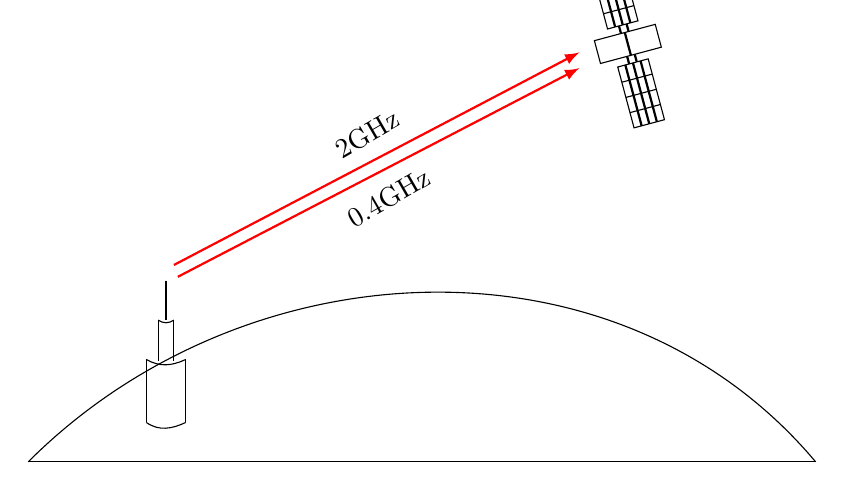
\begin{tikzpicture}
    \coordinate (lend) at (-5, 0);
    \coordinate (rend) at (5, 0);
    \draw (lend) to (rend);
    \draw (lend) to[out=45,in=-230] (rend);

    \coordinate (blb) at (-3.5, 0.5);
    \coordinate (brb) at (-3, 0.5);
    \draw (blb) to[out=-35,in=205] (brb);

    \coordinate (mlb) at (-3.5, 1.3);
    \coordinate (mrb) at (-3, 1.3);
    \draw (mlb) to[out=-30,in=205] (mrb);
    %\draw (mlb) to[out=35,in=-205] (mrb);
    \draw (blb) to (mlb);
    \draw (brb) to (mrb);
    
    \coordinate (tlb) at (-3.35, 1.8);
    \coordinate (trb) at (-3.15, 1.8);
    \draw (tlb) to[out=-35,in=215] (trb);
    \draw (tlb) to (-3.35, 1.28);
    \draw (trb) to (-3.15, 1.28);

    \coordinate (ulb) at (-3.26, 2.3);
    \coordinate (urb) at (-3.24, 2.3);
    \draw (ulb) to (-3.26, 1.8);
    \draw (urb) to (-3.24, 1.8);

    \rotatebox{15}{%
    \draw[] (3.5,4.6) rectangle (4.3,4.3);
    % Up panel
    \draw[thick] (3.9,4.3) to (3.9,4.6);
    \draw[thick] (3.85,4.6) to (3.85,4.7);
    \draw[thick] (3.95,4.6) to (3.95,4.7);
    \draw[] (3.7,5.5) rectangle (4.1,4.7);
    % grid
    \draw[thick] (3.8,4.7) to (3.8, 5.5); 
    \draw[thick] (3.9,4.7) to (3.9, 5.5); 
    \draw[thick] (4.0,4.7) to (4.0, 5.5); 
    \draw[] (3.7,4.9) to (4.1, 4.9);
    \draw[] (3.7,5.1) to (4.1, 5.1);
    \draw[] (3.7,5.3) to (4.1, 5.3);
    % Down panel
    \draw[thick] (3.85,4.3) to (3.85,4.2);
    \draw[thick] (3.95,4.3) to (3.95,4.2);
    \draw[] (3.7,3.4) rectangle (4.1,4.2);
    % grid
    \draw[thick] (3.8,3.4) to (3.8, 4.2); 
    \draw[thick] (3.9,3.4) to (3.9, 4.2); 
    \draw[thick] (4.0,3.4) to (4.0, 4.2); 
    \draw[] (3.7,3.6) to (4.1, 3.6);
    \draw[] (3.7,3.8) to (4.1, 3.8);
    \draw[] (3.7,4.0) to (4.1, 4.0);
    }
    
    \coordinate (satant1) at (2.0,  5.2);
    \coordinate (bcnant1) at (-3.15,2.5);
    \coordinate (satant2) at (2.0,  5.0);
    \coordinate (bcnant2) at (-3.10,2.35);
    \draw[thick,red,-latex] (bcnant1) -- node[above=1mm, align=center, black, rotate=30]{2GHz} (satant1);
    \draw[thick,red,-latex] (bcnant2) -- node[below=1mm, align=center, black, rotate=30]{0.4GHz} (satant2);

\end{tikzpicture}

\caption{DORIS System Description}
\label{fig:doris-system-description}
\end{figure}

\subsection{Theoretical Model of Doppler Observations}
According to \cite{lemoine-2016}, we define four basic events:
\begin{enumerate}
    \item beginning of emission of the 1\textsubscript{st} cycle by the emitter, 
    \(\tau_{e1}\) in the proper time scale of the emitter and \(t_1\) in the coordinate 
    time
    
    \item beginning of reception of the the 1\textsubscript{st} cycle by the receiver, 
    \(\tau_{r1'}\) in the proper time scale of the receiver and 
    \(t_{1'}\) in the coordinate time

    \item end of emission of the N\textsubscript{th} cycle by the emitter, 
    \(\tau_{e2}\) in the proper time scale of the emitter and \(t_2\) in the coordinate 
    time
    
    \item end of reception of the N\textsubscript{th} cycle by the receiver, 
    \(\tau_{r2'}\) in the proper time scale of the receiver and 
    \(t_{2'}\) in the coordinate time
\end{enumerate}

During the proper time interval \(\Delta\tau_{r} = \tau_{r2'} - \tau_{r1'}\), 
the receiver has received the \(N_e\) cycles sent by the emitter, with \(N_e = f_e \Delta\tau_e\), 
\(f_e\) being the proper frequency of the emitter. The receiver is also equipped with
an oscilator and during the proper time interval \(\Delta\tau_{r}\) has generated 
a number \(N_r = f_r \Delta\tau_r\) of cycles, \(f_r\) being the proper frequency of the 
receiver.

The Doppler measurement is the count, by the receiver electronics, of the number 
of cycles of difference between \(N_e\) and \(N_r\):
\begin{equation}
    \begin{split}
    N_{DOP} & = N_e - N_r\\
            & = f_e \Delta\tau_e - f_r \Delta\tau_r
    \end{split}
\end{equation}

\emph{In the RINEX files, this Doppler count is the difference between two phase measurements 
done at different time tags in the proper time-scale of the receiver.}

After a series of assumptions and simplifications, we can derive the theoretical 
formula for the Doppler count \cite{lemoine-2016}:
\begin{equation}
    \begin{split}
        \frac{c}{f_e \Delta\tau_r} N_{DOP} & \approx c \frac{f_e - f_r}{f_e} \\
        & - (1 - \frac{U_e}{c^2} - \frac{{V_e}^2}{2 c^2}) \frac{\rho_2 - \rho_1}{\Delta\tau_r}\\
        & + \frac{1}{c} (U_r - U_e + \frac{{V_r}^2 - {V_e}^2}{2}) \\
        & + \frac{2 \mu}{c^2 \Delta\tau_r} [\ln{(\frac{R_1 + R_{1'} + \rho_1}{R_1 + R_{1'} - \rho_1})} - \ln{(\frac{R_2 + R_{2'} + \rho_2}{R_2 + R_{2'} - \rho_2})}]
    \end{split}
\end{equation}

where \(U\) is the gravitational potential, \(V\) is the velocity of the clock, \(R\) 
is the geometric distance and \(\rho\) is the curvlinear trajectory (of the photon(s)).

The above equation can be (arbitrarily) split into two parts, one containing the ``measured'' 
quantities and one with the ``theoretical'' terms, as \cite{lemoine-2016}:
\begin{subequations}\label{eq:lem12}
  \begin{align}
    u_{measured} & = \frac{c}{f_e} (f_e - f_r -
     \frac{N_{DOP}}{\Delta\tau_r}) + \Delta u_{REL} \label{eq:lem12a} \\
    u_{theo}     &= \frac{\rho_2 - \rho_1}{\Delta\tau_r} (1- \frac{U_e}{c^2} - 
      \frac{{V_e}^2}{2 c^2}) \label{eq:lem12b}
  \end{align}
\end{subequations}

with
\begin{equation}
    \begin{split}
        \Delta u_{REL} &= \frac{1}{c} (U_r - U_e + \frac{{V_r}^2 - {V_e}^2}{2}) \\
        & + \frac{2 \mu}{c^2 \Delta\tau_r} [\ln{(\frac{R_1 + R_{1'} + \rho_1}{R_1 + R_{1'} - \rho_1})} - \ln{(\frac{R_2 + R_{2'} + \rho_2}{R_2 + R_{2'} - \rho_2})}]
    \end{split}
\end{equation}

We now need to introduce some additional corrections:
\(\Delta u_{IONO}\) and \(\Delta u_{TROPO}\), are the propagation corrections of 
the radio electric signal through the ionosphere and troposphere respectively. 

Additionaly, in the actual case (measurements), the nominal frequencies \(f_e\) and \(f_r\) 
are not the ``true'' ones; we hence need to apply a relative correction (e.g. for the 
emmiter) \(f_{e_T} = f_{e_N} (1 + \frac{\Delta f_e}{f_{e_N}})\), where the subscript \(T\) 
denotes the ``True'' frequency and \(N\) the nominal one. Thus in \ref{eq:lem12} the 
terms \(f_e\) and \(f_r\) need to be substituted by \(f_{e_T}\) and \(f_{r_T}\) respectively.

We will place \(\Delta u_{IONO}\) and \(\Delta u_{REL}\) (which do not involve adjusted parameters) 
on the ``measured'' part of \ref{eq:lem12} and \(\Delta u_{TROPO}\) and \(\frac{\Delta f_e}{f_{e_N}}\) 
on the ``theoretical'' part; neglecting some minor terms, we reach the equation \cite{lemoine-2016}:
\begin{subequations} \label{eq:lem13}
    \begin{align}
        u_{measured} & = \frac{c}{f_{e_N}} (f_{e_N} - f_{r_T} -
          \frac{N_{DOP}}{\Delta\tau_r}) + \Delta u_{REL} + 
          \Delta u_{IONO} \label{eq:lem13a} \\
        u_{theo} &= \frac{\rho_2 - \rho_1}{\Delta\tau_r} 
          (1- \frac{U_e}{c^2} - \frac{{V_e}^2}{2 c^2}) + 
          \Delta u_{TROPO} - \frac{c(\frac{N_{DOP}}{\Delta\tau_r} + 
          f_{r_T})}{f_{e_N}} \frac{\Delta f_e}{f_{e_N}} \label{eq:lem13b}
    \end{align}
\end{subequations}

where 
\begin{itemize}
    \item \(u_{measured}\) is the measured relative velocity between the emitter and 
    the receiver between the events 1' and 2', based on the Doppler count \(N_{DOP}\), 
    corrected for the ionospheric and relativistic effects.

    \item \(u_{theo}\) is the the theoretical (computed) emitter/receiver relative velocity 
    between the events 1' and 2', corrected for the tropospheric effect and for a solved-for 
    frequency bias \(\frac{\Delta f_e}{f_{e_N}}\) of the emitter. \(f_{r_T} = f_{r_N} (1 + \frac{\Delta f_r}{f_{r_N}})\) 
    is an estimate of the proper frequency of the receiver.

    \item \(\Delta u_{REL} = \Delta u_{{REL}_c} + \Delta u_{{REL}_r}\) is the relativistic 
    correction, composed of two parts: the clock correction \(\Delta u_{{REL}_c}\) and the 
    travel correction \(\Delta u_{{REL}_r}\)
    \begin{subequations} \label{eq:lem14}
        \begin{align}
            \Delta u_{{REL}_c} & = \frac{1}{c} 
              (U_r - U_e + \frac{{V_r}^2 - {V_e}^2}{2}) \label{eq:lem14a}\\
            \Delta u_{{REL}_r} & = \frac{2 \mu}{c^2 \Delta\tau_r} \left[ 
              \ln{(\frac{R_1 + R_{1'} + \rho_1}{R_1 + R_{1'} - \rho_1})} - 
              \ln{(\frac{R_2 + R_{2'} + \rho_2}{R_2 + R_{2'} - \rho_2})} \right] \label{eq:lem14b}
        \end{align}
    \end{subequations}
\end{itemize}

Note that \ref{eq:lem13} can be further simplified to \ref{eq:lem17} by 
ommiting small terms (\ref{ssec:small-terms}).

\emph{Usually, one frequency offset and one tropospheric zenithal bias are adjusted per pass.}

\subsection{Implementation of the Doppler Observation Model}

\subsubsection{Small Terms}
\label{sssec:small-terms}

In \ref{eq:lem13}, the smallest terms are \(-U_e / c^2 - {V_e}^2 / 2 c^2\) and 
\(\Delta u_{{REL}_T}\); in the case of DORIS they ammount to \num{11.} and 
\num{6.} \SI{10e-6}{\meter\per\second} respectively (\cite{lemoine-2016}). 
Furthermore, since the emitters are located on the ground, the term 
\(-U_e / c^2 - {V_e}^2 / 2 c^2\) is constant per station. This small 
relativistic offset is absorbed by the adjustment of \(\Delta f_e / f_{eN}\). 
So it is possibly to furher simplify \ref{eq:lem13} to:
\begin{subequations} \label{eq:lem17}
    \begin{align}
        u_{measured} & = \frac{c}{f_{e_N}} (f_{e_N} - f_{r_T} -
          \frac{N_{DOP}}{\Delta\tau_r}) + 
          \Delta u_{{REL}_C} + \Delta u_{IONO} \label{eq:lem17a}\\
        u_{theo} &= \frac{\rho_2 - \rho_1}{\Delta\tau_r} + \Delta u_{TROPO} - 
          \frac{c(\frac{N_{DOP}}{\Delta\tau_r} + f_{r_T})}{f_{e_N}} 
          \frac{\Delta f_e}{f_{e_N}} \label{eq:lem17b}
    \end{align}
\end{subequations}

\subsubsection{Correction of Aberration}

\subsubsection{Geopotential}
For a station on the geoid, the potential at the level of the station is the sum 
of the gravitational potential and the centrifugal potential due to the Earth's 
rotation: \(U_{GEO} = U_e + \frac{{V_e}^2}{2}\), which is a constant. For a station 
not located on the geoid, the quantity \(U_e + \frac{{V_e}^2}{2}\) will only depend 
on the height of the beacon above the geoid.

For the computation of the gravitational potential for \gls{leo} satellites, 
the pottential \(U_r\) cannot be restricted to the central term only and we must 
take into account the \(J_2\) term (at least, in addition to \(\mu / r\). The formula 
for the computation of the potential in this case is \cite{lemoine-2016}:
\begin{equation}
  \label{eq:lem18}
  U_r = \frac{\mu}{r} \left( 1- \left(\frac{\alpha_\Earth}{r}\right)^2 
    J_2 \frac{3 sin^2(\phi) - 1}{2} \right)
\end{equation}
with \(\alpha_\Earth\) the equatorial radious of the earth, \(r\) radial 
distance of the satellite (to the Earth's center), \(\phi\) latitude of the 
satellite and \(J_2 = 1.0826359 \dot 10^{-3}\) in the zero-tide system.

\subsubsection{True Proper Frequency of the Receiver}
\label{sssec:true-proprtfrequency-of-the-receiver}

For the term \(f_{r_T}\) that appears in \ref{eq:lem13}, we need an estimate of \(\Delta f_{r} / f_{r_N}\). 
This estimate can be obtained in one of the following ways \cite{lemoine-2016}:
\begin{enumerate}
    \item via the field ``F'' recorded for every single measurement in the DORIS 
    RINEX file (see \ref{ssec:relative-frequency-offset}); not that this estimation 
    is not very smooth, as noticed by \cite{GAO2015} and it is advisable, before 
    using it in \ref{eq:lem13}, to perform a linear (or polynomial) regression of 
    these estimates over one or a few days.

    \item It can also be obtained from a polynomial regression
    over the frequency offsets estimated during the passes
    over the master beacons

    \item It can finally be estimated by the users themselves as a
    by-product of their re-computation of the timetagging polynomial (see \cite{MERCIER2010})
\end{enumerate}

\subsection{Nominal Receiver \& Emitter Frequencies}
\label{ssec:nominal-frequencies}
In the observation equation model \ref{eq:lem13} we distinguish between 
\emph{nominal} and \emph{true} receiver/emitter frequencies, to account for 
the fact that in ``real world'' these two are not actually equal.

\subsubsection{Emitter/Beacon Nominal Frequencies, $f_{e_N}$}
\label{sssec:beacon-nominal-frequencies}

RINEX file headers, contain values of the \emph{station frequency shift 
factor} $k$ for each of the beacons involved (\cite{DORISRNX3}, Sec. 6.16). 
These are used to compute the ``nominal'' frequencies of the beacon/emitter. 
(usually, this shift factor is just $0$, but it can be an integer 
$k \neq 0$). The frequencies are computed as (\cite{DORISRNX3}, Sec. 6.16):
\begin{equation}
  \begin{aligned}
    L_{2GHz}   &= 543 \cdot F_0 \left( \frac{3}{4} + \frac{87\cdot k}{5 \cdot 2^{26}} \right) \\
    L_{400MHz} &= 107 \cdot F_0 \left( \frac{3}{4} + \frac{87\cdot k}{5 \cdot 2^{26}} \right) 
    \label{eq:nominal-freq}
  \end{aligned}
\end{equation}
where $F_0 = 5e6 \text{ Hz}$ the USO frequency. These value, are the ones 
labelled as $f_{e_N}$ in \ref{eq:lem13}.

The \emph{true proper frequency} of the emitter $f_{e_T}$, can be computed 
from:
\begin{equation}
  f_{e_T} = f_{e_N} \cdot \left( 1 + \frac{\Delta f_e}{f_{e_N}} \right)
\end{equation}
but the quantity $\Delta f_e / f_{e_N}$ is not know a-priori and has to be 
estimated during the processing.

We estimate $\Delta f_e / f_{e_N}$ using a \colorbox{blue!20}{linear model using proper time}, 
aka $\frac{\Delta f_e}{f_{e_N}}\at{\tau=\tau _i} = \alpha + \beta \cdot \delta \tau$
with an a-priori value of 0 and no process noise. For the estimation, we need 
the partials of the observation equation \ref{eq:lem13b} w.r.t. the $\alpha$ and 
$\beta$ parameters, which are:
\begin{equation}
  \begin{aligned}
  \frac{\partial v_{theo}}{\partial \alpha} &= 
    \frac{c(\frac{N_{DOP}}{\Delta\tau_r} + f_{r_T})}{f_{e_N}} \\
  \frac{\partial v_{theo}}{\partial \beta} &= 
    \frac{c(\frac{N_{DOP}}{\Delta\tau_r} + f_{r_T})}{f_{e_N}} \cdot \delta \tau
  \end{aligned}
\end{equation}

\subsection{Receiver True Proper Frequency $f_{r_T}$}
\label{ssec:receiver-true-proper-frequency}
In equation \ref{eq:lem13}, $f_{r_T}$ is the \emph{true proper frequency of 
the receiver} with nominal value 
\begin{equation}
  f_{r_T} = f_{r_N} \cdot \left( 1 + \frac{\Delta f_r}{f_{r_N}} \right)
\end{equation}
where $f_{r_N}$ is the ``nominal'' frequency value.

In practice the value $\Delta f_r / f_{r_N}$, called the \emph{relative 
frequency offset} of the receiver, is given in the RINEX files for each epoch 
(under the observable tagged \texttt{F}). Note that these values are scaled to 
$10^{-11}$ (\cite{DORISRNX3}, Sec. 6.11), so that for a given epoch $t_i$, the 
true frequency is
\begin{equation}
  f_{r_T}\at{t=t_i} = f_{r_N} \cdot \left( 1 + F_{t_i} \cdot 10^{-11} \right)
  \label{eq:tpf-rec}
\end{equation}
where $F_{t_i}$ is the relative frequency offset value recovered from the RINEX 
file.

In our implementation, we use ``smoothed'' values of RINEX-provided 
$\Delta f_r / f_{r_N}$ estimates. In a first step/pass we use a linear model 
to filter all the values in the RINEX file (as suggested by \cite{lemoine-2016}, 
Sec. 2.5.4). We then use this linear model to compute relative frequency offset 
values when needed. 

\subsection{Coordinate \& Proper Time}
\label{ssec:coordinate-proper-time}
We use TAI as coordinate time; to transform RINEX observation time (given in 
proper time $\tau$) to coordinate time $t$, we use the \emph{receiver clock 
offset} values, extracted from the RINEX file (one value per observation block).

Hence, if an observation block is taged at proper time $\tau _i$ at the RINEX 
file, and the receiver clock offset for this block is $\Delta \tau _i$ (again from 
RINEX), then the coordinate time of the event in TAI is:
\begin{equation}
  t^{TAI}_i = \tau _i + \Delta \tau _i
\end{equation}

\subsection{Tropospheric Correction}
\label{ssec-tropospheric-correction}

\subsubsection{Mapping Functions}
We use the GPT3/VMF3 (\cite{Landskron2018}) to handle tropospheric refraction. 
Given the elevation angle $el$ and the beacon's ellipsoidal coordinates 
$\bm{r}=\begin{pmatrix} \lambda & \phi & h\end{pmatrix}$, we use the \texttt{gpt3} 
$\ang{5} \times \ang{5}$ grid to interpolate the $ah$ and $aw$ coefficients; 
we then compute the mapping function (with height correction) $mf_{wet}$ and 
$mf_{hydrostatic}$.

\subsubsection{Zenith Delays}
For the hydrostatic zenith delay $zd_{hydrostatic}$ we use the ``refined'' 
\emph{Saastamoinen} model (\cite{Davisetal85} and \cite{Saastamoinen72}). 
The corresponding value for the wet delay, $zd_{wet}$ is estimated during the 
analysis, \emph{per beacon and per pass}, using an initial value provided by 
\cite{Askneetal87}.

\subsubsection{Tropospheric Correction}
Using the mapping function and the zenith delay, we derive the tropospheric 
delay for an observation at $t=t_i$, given by:
\begin{equation}
  \delta _{TRO} [\si{\m}] = zd_{hydrostatic} \cdot mf_{hydrostatic} + zd_{wet}\at{t=t_i} \cdot mf_{wet}
  \label{eq:tropo-delay}
\end{equation}

The tropospheric correction term in \ref{eq:lem13}, is actually the ``time-differenced'' 
tropospheric delay between two measurements (the same ones used to derive the 
Doppler count), given in \si{\m \per \s}. That is:
\begin{equation}
  \begin{aligned}
    \Delta v_{TROPO} [\si{\m \per \s}] 
      &= \left( \delta _{TRO} \at{t=t_{i-1}} - \delta _{TRO} \at{t=t_{i}} \right) / \Delta \tau\\
      &= \left( \left[ zd_{h} \cdot mf_{h} + zd_{w}\at{t=t_{i-1}} \cdot mf_{w} \right]\at[\big]{t=t_i} - 
        \left[ zd_{h} \cdot mf_{h} + zd_{w}\at{t=t_{i-1}} \cdot mf_{w} \right]\at[\big]{t=t_{i-1}} \right) \ \Delta \tau
    \label{eq:dtrop-diff}
  \end{aligned}
\end{equation}

Note that in the above equation we use the same value $zd_{w}\at{t=t_{i-1}}$ 
for the wet part of the zenith delay, that is the best estimate prior to 
incorporating the (new) measurement at $t=t_i$.

The parameter $zd_{w}$ is estimated using no constraints and a simple white 
noise model (no process noise). Since it is an estimated parameter, we need 
to compute the (partial) derivative of the observation equation w.r.t to it, 
that is:
\begin{equation}
  \frac{\partial v_{theo}}{\partial zd_{w}} = \frac{mf_{w}\at[\big]{t=t_i} 
    - mf_{w}\at[\big]{t=t_{i-1}}}{\Delta \tau}
  \label{eq:partials-zwd}
\end{equation}

\subsection{Ionospheric Correction}
\label{ssec:iono-correction}
The basic observation equation \ref{eq:lem13}, is formed for the \SI{2}{\GHz} 
carrier. For each measurement, we have to account for the ionospheric path 
delay, by computing a correction (in cycles) as (\cite{lemoine-2016}, Sec. 2.5.7):
\begin{equation}
  \delta_{ION} [\SI{2}{\GHz}\text{ cycles}] = 
    \frac{L_{\SI{2}{\GHz}} - \sqrt{\gamma} \cdot L_{\SI{400}{\MHz}}}{\gamma - 1}
  \label{eq:iono-delay-cycles}
\end{equation}

which is added to the \SI{2}{\GHz} measurement at time $t=t_i$ (obtained by the 
RINEX file). Thus, the corrected observation is:
\begin{equation}
  L_{\SI{2}{\GHz},IF} [\SI{2}{\GHz}\text{ cycles}] = 
    L_{\SI{2}{\GHz}} + \delta_{ION}
  \label{eq:l2if}
\end{equation}

Note that after applying \ref{eq:l2if}, we should refer to the ``Iono-Free'' 
geometrical endpoints of the observations (and not the \SI{2}{\GHz} endpoints). 
This means that we have to apply respective \emph{phase center} corrections 
both at the satellite and at the beacon.

When applied to \ref{eq:lem13}, we have to ``differenciate'' the ionospheric 
delay computed from \ref{eq:iono-delay-cycles}, affecting two observations 
(the same ones used to derive the Doppler count). Hence, the term 
$\Delta v_{IONO}$ appearing in \ref{eq:lem13} is:
\begin{equation}
  \Delta v_{IONO} [\si{\m \per \s}] = 
    \tikz[baseline]{
      \node[fill=blue!20,anchor=base](en1){$\frac{c}{f_{e_N}}$};
    }
    \cdot 
    \frac{\delta_{ION}\at[\big]{t=t_{i-1}} 
    - \delta_{ION}\at[\big]{t=t_i}}{\Delta \tau}
  \label{eq:dion-diff}
\end{equation}

\subsubsection{2GHz \& Iono-Free Phase Center}
\label{sssec:2ghz-ionofree-pco}
To get to the iono-free phase center from the beacon \gls{arp}, 
we use (\cite{lemoine-2016}, Sec. 2.5.7, Eq. 20):
\begin{equation}
  \bm{r}_{iono-free} = \bm{r}_{\SI{2}{\GHz}} + \frac{\bm{r}_{\SI{2}{\GHz}} 
    - \bm{r}_{\SI{400}{\MHz}}}{\gamma - 1}
  \label{eq:ionf-pco}
\end{equation}

where $\bm{r}_{\SI{2}{\GHz}}$ and $\bm{r}_{\SI{400}{\MHz}}$ are the 
eccentricities of the \SI{2}{\GHz} and the \SI{400}{\MHz} carriers respectively 
from the beacon antena phase center (given eg at \cite{DORISGSM}, Sec. 5.2.1).

Note that in \ref{eq:ionf-pco}, the eccentricity vector $\bm{r}_{iono-free}$ 
is in a topocentric RF. Hence, to compute the ECEF coordinates of the 
iono-free phase center, given that we have the ECEF coordinates of the beacon's 
\gls{arp} $\bm{r}_{arp}$ (see \ref{ssec:beacon_coordinates}), we use:
\begin{equation}
  \bm{r}^{ecef}_{iono-free} = \bm{r}_{arp} + \bm{R}^T \cdot \bm{r}_{iono-free}
  \label{eq:arp-to-if-pc}
\end{equation}
where $\bm{R}$ is the cartesian-to-topocentric rotation matrix, computed 
at $\bm{r}_{arp}$.

In accordance to the beacons, a similar geometric reduction must be applied 
at the satellite's end, to correct for the discrepancy between the \SI{2}{\GHz} 
and the \emph{iono-free} phase center:
\begin{equation}
  \bm{r}^{satf}_{iono-free} = \bm{r}^{satf}_{\SI{2}{\GHz}} + 
    \frac{\bm{r}^{satf}_{\SI{2}{\GHz}} - 
    \bm{r}^{satf}_{\SI{400}{\MHz}}}{\gamma - 1}
\end{equation}

where the superscript $satf$ denotes the \emph{satellite-fixed} body/reference 
frame. On-board satellite antenna phase center offset values can be found in 
\cite{DorisSatModels}.

\subsubsection{Relativistic Correction}
\label{sssec:relativistic-correction}
\ref{eq:lem13} contains a relativistic correction term, $\Delta u_{REL}$. This 
correction is plit into two parts, $\Delta u_{REL_c}$ the part containing the 
clock correction and $\Delta u_{REL_r}$, containing the effect of the travel 
path. Here, we are only considering the $\Delta u_{REL_c}$ part.

The correction is computed (for a given obserbation) from the formula:
\begin{equation}
  \Delta u_{REL_c} = \frac{1}{c} \left( U_r - U_e + \frac{V^2_r - V^2_e}{2} \right) \si{\m}
  \label{eq:lem14}
\end{equation}
For the receiver part, the respective quantities in \ref{eq:lem14} are given by:
\begin{equation}
  \begin{aligned}
    V^2_r &= \norm{\bm{v}_{ecef}}^2 \\
    U_r   &= \frac{\mu}{\norm{\bm{r}_{ecef}}} \cdot \left( 1 - 
      \left(\frac{\alpha}{\norm{\bm{r}_{ecef}}}\right) ^2 \cdot J_2 \cdot
        \frac{3 \cdot \sin ^2{\phi} -1}{2} \right)
  \end{aligned}
  \label{eq:potential-receiver}
\end{equation}
where $\bm{r}_{ecef}$ and $\bm{v}_{ecef}$ are the position and velocity of the 
satellite at the given instant, in the terrestrial RF, aka ITRF.

For the emitter, things are further simplified. We consider $V_e = 0$ and the 
potential is computed as 
\begin{equation}
  U_e = \frac{\mu}{\norm{\bm{r}_{ecef}}}
  \label{eq:potential-emitter}
\end{equation}
where $\bm{r}_{ecef}$ is the position of the beacon in ITRF.

In \ref{eq:lem13}, we need the ``differentiated'' relativistic corrections, thus 
\begin{equation}
  \label{eq:drel-diff}
  \begin{aligned}
    \Delta v_{REL} &= \frac{1}{c} \left( \left[ U_r - U_e + \frac{V^2_r - V^2_e}{2} \right]\at{t=t_i} - \left[ U_r - U_e + \frac{V^2_r - V^2_e}{2} \right]\at{t=t_{i-1}} \right) \\
      &= \frac{1}{c} \cdot \left( U_r\at{t_i} - U_r\at{t_{i-1}} +  \frac{V_r\at{t_i}-V_r\at{t_{i-1}}}{2} \right) \si{\m\per\s}
  \end{aligned}
\end{equation}
